\documentclass{article}
\usepackage[utf8]{inputenc}
\usepackage{graphicx}
\usepackage{amsmath}
\usepackage{amssymb}
\usepackage{todonotes}
\usepackage{appendix}
\usepackage{mavlab}
\usepackage{times}
\usepackage{siunitx}
\usepackage{multirow}
\usepackage{tabularx}
\usepackage{svg}
\usepackage{float}
\usepackage{booktabs} % For better horizontal lines
\usepackage{lipsum}   % Optional: for sample text filling the document
\usepackage{makecell}  % Add this in your preamble
\usepackage{array}  % Ensure this is in your preamble
\usepackage{hyperref}

\title{Exploring sparsity performance gain in a spiking convolutional neural network for optical flow estimation}
\author{E. Lucassen\thanks{Email address: elucassen@student.tudelft.nl} \\ Delft University of Technology, Kluyverweg 1, Netherlands}

\begin{document}
\maketitle
\begin{abstract}
	Event cameras present a novel approach for vision-based sensing by providing pixel values based on changes in brightness levels. Such data is inherently sparse and allows for potential speedups on the convolution operator by reducing the reducing the number of operations. Conventional engines such as TorchSparse \cite{tang2023torchsparse++} and Minkowski-Engine \cite{choy20194d-MinkowskiEngine} suffer from long hashing times in creating maps of the required kernel operations. Minuet \cite{yang2023minuet} aims to decrease these hashing times but is ultimately still slower than the dense counterpart for the 85\% sparse Evimo2 dataset. For several specific circumstances related to the degree of sparsity, the number of filter channels or change in dimensionality, using sparse convolutions may provide performance enhancements compared to their dense counterpart. 
	\end{abstract}


\section{Introduction}
\label{Background}

% Overview of event cameras and their output characteristics.
Event cameras are neuromorphic sensors that activate pixels once a threshold change in brightness is exceeded. This contrasts with conventional cameras, which capture all pixels simultaneously across the field of view (or rapidly ascending vertical bars in the case of rolling shutters). Conventional cameras typically output in RGB (Red-Green-Blue) or YUV (Brightness-Colour), while event cameras produce two channels: activations and deactivations (negative changes in brightness).

% Introduction to the dataset used and its sparsity characteristics.
The data is from EVIMO2, a collection of indoor datasets generated using event cameras \cite{EVIMO2}. Since only pixels with changing brightness activate, the output is inherently sparse. An overview of the sparsity levels for one full epoch of the dataset is given in figure \ref{Sparse_histogram}, showing an average sparsity of 85\%.

\begin{figure}
    \centering
    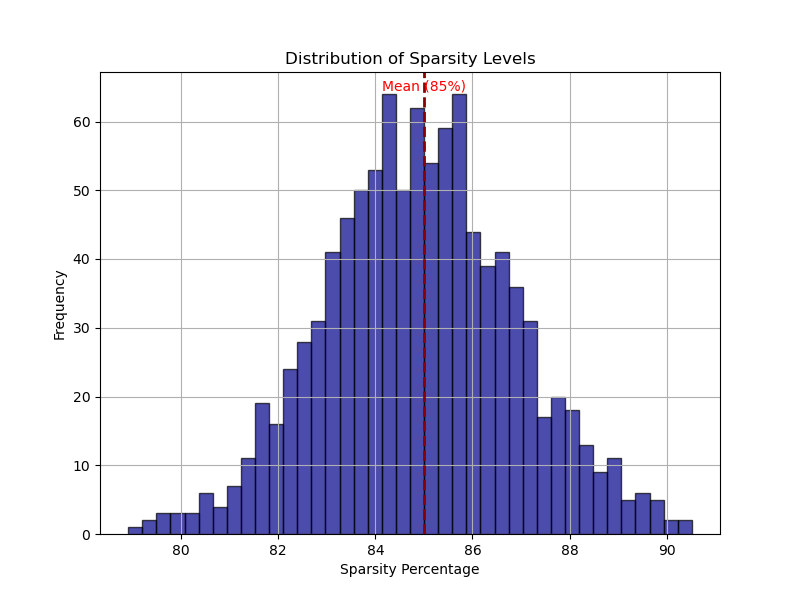
\includegraphics[width=0.9\linewidth]{figures/Sparse_histogram.png}
    \caption{Histogram of sparsity percentages across the entire dataset}
    \label{Sparse_histogram}
\end{figure}

% Description of the primary research question and the network under investigation.
The primary network examined is based on the work of \cite{hagenaars2021self}. This research investigates whether speedups can be achieved in fundamental building blocks—3D convolution, concatenation, and upsampling—using the EVIMO2 dataset. Achieving such speedups would enable the construction of faster networks leveraging sparsity. All experiments were conducted on a Nvidia A100 80GB GPU, with detailed system hardware specifications provided in Appendix A.

% Explanation of the main operation considered and its implementation.
The main operation considered is 3D convolution, implemented in Pytorch using the im2col algorithm and GEMM (General Matrix Multiplication), both executed in CUDA, an extension of C++ developed by Nvidia as the primary framework for deep learning. Python serves merely as a wrapper, with underlying operations in C++.

% Discussion on various approaches for sparsity and relevant benchmarks.
Sten focuses on sparsifying inputs and weights, while DeepML is designed for rapid inference of sparse networks. However, GPUs are optimized for parallel, simultaneous computation, often making dense multiplications more efficient than sparse ones \cite{ivanov2023sten}. \cite{hosseini2022sparse-benchmark} benchmarked torch.sparse, and \cite{nikdan2023sparseprop} discussed more efficient backpropagation.

% Impact of conventional dense convolutions on sparsity and introduction of submanifold sparse convolutions.
In conventional dense convolutions, the activation kernel slides across the entire grid, resulting in a significantly less sparse output feature map compared to the input. The example provided by the paper is illustrated in figure \ref{decrease-sparsity}. For the network under investigation, average input sparsity of 95\% in the first layer decreases rapidly to 50\% and 10\% in subsequent layers, depending on the kernel size. Submanifold sparse convolutions were introduced by \cite{SubmanifoldSparseConvNet} to address this issue, ensuring convolutions are performed only on active input sites, maintaining the same degree of sparsity throughout the network.

\begin{figure}[h!]
    \centering
    
\includegraphics[width=0.9\linewidth]{figures/Sparse.png}
    \caption{Decrease in sparsity when using conventional convolutions \cite{SubmanifoldSparseConvNet}}
    \label{decrease-sparsity}
\end{figure}

% Capabilities of Pytorch for creating sparse tensors and its limitations.
Pytorch allows the creation of sparse tensors in various formats such as CSR, COO, and BSR, and supports basic operations like transpose, resize, and matmul (XX cite website). However, as of this writing, neither submanifold nor standard sparse convolutions are supported.

% Development of libraries to support submanifold convolutions and their improvements.
Various libraries have been developed by different groups to support submanifold convolutions. These libraries typically build a hash table based on active input indices and kernel size, creating a map of necessary GEMM (General Matrix Multiplication) operations. This process significantly reduces the number of floating point operations (FLOPS) required by the network. The Minkowski engine was first introduced by \cite{choy20194d-MinkowskiEngine}, followed by contributions from Facebook \cite{SubmanifoldSparseConvNet}, \cite{focalsconv-chen-SPconvPlus}, and Torchsparse++ \cite{tang2023torchsparse++}. These libraries have undergone various improvements, such as more efficient hash-map generation and better utilization of available computation resources. Recently, Minuet was introduced, claiming faster mapping by replacing hash-table creation with a custom binary search algorithm \cite{yang2023minuet}, addressing some issues present in earlier engines.

% Use of CUDA in sparse libraries for efficient data processing and tensor operations.
All these sparse libraries utilize CUDA, a programming extension to C++ developed by Nvidia since 2006, aimed at providing efficient data flow and tensor operation processing. These libraries are implemented using CUDA and are subsequently profiled.

\section{Methodology \& Network Analysis}
\label{Methodology}

% Performance analyzed by profiling CPU and CUDA kernels to identify optimization opportunities using sparsity.
Performance was analyzed by profiling CPU and CUDA kernel operations to determine optimization opportunities using sparsity. The focus was primarily on the forward pass, as it required the most computation time, with potential speedups being relevant for inference as well. To address the research question, several sub-questions were formulated.

\subsection{Profiling}

% Explanation of the profiling method and the choice of CUDA events for accuracy.
Profiling the execution speed of Python functions commonly uses `time.time()`. However, for GPU inference, it is better to measure CUDA events while ensuring GPU synchronization. This method was chosen for accuracy.

% Importance of GPU warm-up and the approach taken to ensure accurate timing measurements.
Proper GPU warm-up is crucial; initial execution times are longer. Therefore, the first 10 measurements were discarded, and subsequent steps were evaluated over one full epoch. Data loading overhead was excluded, focusing only on the `model(x)` function's execution time.

% Conversion of input data to sparse tensors and its exclusion from profiling.
When using sparse convolutions, input conversion to sparse tensors is necessary. This conversion was assumed to be a one-time process during data preparation, thus excluded from profiling.

% Use of PyTorch profiler for detailed analysis and the need for caution due to overhead.
Detailed analysis of operations was performed using the PyTorch profiler, which can generate flamegraphs showing the time taken by each step. However, the profiler introduces overhead, requiring caution when comparing CUDA event timings.

% Importance of resetting the cache for sparsity engines to ensure accurate mapping step measurements.
For sparsity engines, the mapping step is critical. A single forward pass reuses previously generated hashmaps, speeding up subsequent steps. Therefore, it is essential to reset the cache and force the network to remap operations when recording compute times.

% Consistency in running all networks for one full epoch to ensure comparable inputs.
All networks with the investigated parameters were run for one full epoch across the entire dataset to ensure cumulative inputs remained consistent.

\subsection{Input Data}

% Pre-processing of input tensors and conversion to sparse format before training.
In the original network, input tensor concatenation was performed during the forward pass. This step is now performed beforehand for consistency. Sparse tensors are created by finding the indices of nonzero input tensors using the `torch.nonzero()` function.

% Detailed explanation of creating sorted arrays for coordinates and values based on input types.
The value dimension at each coordinate depends on the input type, with single entries for grayscale images, three for RGB data, and one or two for event camera outputs. For each batch, a sorted array is made for the coordinate and value tensors of dimension \([x, 3]\) and \([x, 2]\) with \(x\) being the number of nonzero elements for that batch, and the depth, height, width dimensions for the coordinates, and the number of channels for the value array.

% Concatenation of batches and provision as input for SparseTensor object.
These batches are then concatenated and provided as input for the SparseTensor object as specified by the various sparsity libraries. It should be noted that this process incurs significant computational costs and is assumed to be performed during the data preparation step before training. The validity of this assumption will be discussed in Section 5.

\subsection{Network Architecture}

% Description of the network architecture following a U-net structure with specific modifications.
The network architecture follows a U-net structure with downsampling, a bottleneck layer, concatenation with the input, and upsampling based on \cite{hagenaars2021self}. Since Torchsparse and Minuet do not support bilinear/nearest neighbor upsampling, 3D transposed convolutions are used for fair comparison.

\begin{table}[H]
    \centering
    \begin{tabular}{|c|c|c|c|c|}
        \hline
        Operation & stride & Input - Output dim & Activation \\
        \hline
        3D convolution   & 2 & [2] $\rightarrow$ [16] & ReLU   \\
        3D convolution   & 2 & [16] $\rightarrow$ [32] & ReLU \\
        3D convolution & 2 & [32] $\rightarrow$ [32] & ReLU \\
        Concatenation & [-] & [32] $\rightarrow$ [48] & ReLU  \\
        3D T convolution & 2 &[48] $\rightarrow$ [16] & ReLU \\
        3D T convolution & 2 & [48] $\rightarrow$ [16] & ReLU \\
        Prediction layer & 1 & [16] $\rightarrow$ [2] & Tanh \\
        \hline
    \end{tabular}
    \caption{Performance and Memory Usage by Kernel Size}
    \label{tab:kernel_performance}
\end{table}

\begin{table}[ht]
    \centering
    \begin{tabular}{|c|c|c|c|}
        \hline
        Layer & Min Time & Max Time & Avg Time \\
        \hline
        Combined   & 0.81 & 2.54 & 0.848  \\
        e1   & 0.196 & 0.645 & 0.236 \\
        e2 & 0.170 & 1.66 & 0.194  \\
        d2 & 0.106 & 0.336 & 0.134  \\
        d2-int & 0.00921 & 0.233 & 0.029  \\
        d1 & 0.125 & 0.368 & 0.145  \\
        d1-int & 0.0205 & 0.213 & 0.0306  \\
        p1 & 0.164 & 0.396 & 0.192  \\
        \hline
    \end{tabular}
    \caption{Profiling of network layers, in milliseconds}
    \label{tab:kernel_performance}
\end{table}

% Profiling results showing negligible time differences for non-convolutional operations.
Beyond 3D convolutional and activation layers, a typical network architecture might include concatenations and batch normalization. Profiling revealed negligible time differences between dense and sparse architectures for these operations. Activation functions and concatenations consistently executed within microseconds, as did batch normalization operations, making them too rapid to significantly impact overall execution time. Therefore, this study emphasizes the computational cost of convolutional operations instead.



\section{Results}
\label{Results}
The results of the profiling are given in this chapter. The results are for a network that receives an input of size BxCxDxHxW with B the batch size, C the number of channels (which is 2 for the Evimo dataset; activations and deactivations), D the temporal depth, H the height and W the width. The height, width and channels always remains 128, 128 and 2 respectively, with the temporal depth and batch size as user-defined parameters. 

\subsection{Network analysis}
First, an analysis was made of the computational times throughout the network layers. It should be noted that CUDA XX. Synchronize needs to be called before each operation whereas normally the GPU can perform some of these operations in parallel. Thus the combined compute time will be higher than normal, but this serves as a rough overview of how much time is spent on each layer proportionally. Figure \ref{tab:kernel_performance} shows the results. In figure \ref{flamegraph-execution} it can be seen that roughly an equal amount of time is spent throughout each layer, with a slight reduction in execution time for the layers of reduced dimensionality. Furthermore, the sparsity quickly reduces from 85\% at the input to around 50\% after the first layer and remaining at this value due to the ReLU activation blocks. The fact that computation times are roughly equal for each convolutional operation, in combination with the fact that for conventional convolution the sparsity of the input propagated throughout the network rapidly decreases, reinforces the premise that submanifold convolutions are necessary for achieving a speedup in computational times. 

% \begin{figure*}[h!]
%   \centering
%   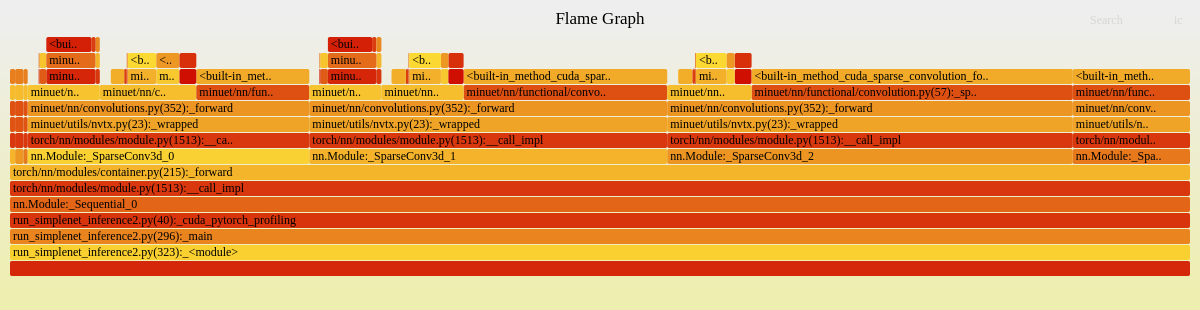
\includegraphics[width=0.95\linewidth]{figures/minuet_img.png}
%   \caption{Execution times throughout network}
%   \label{flamegraph-execution}
% \end{figure*}



\subsection{Torchsparse \& Minuet}
The initial library under study, TorchSparse, was deemed unsuitable for the research network primarily due to the excessive time consumed during the mapping step. In this step, a sorted index is created to map the necessary operations, significantly slowing down the process compared to its dense counterparts. Moreover, while a single mapping step suffices for networks with uniform stride, networks requiring changes in filter dimensions necessitate additional mapping operations. To illustrate, two flamegraphs are included that compare the computational overhead of mapping in a standard network versus a U-net, highlighting the inefficiencies introduced by dimensional changes in filters. 

During the course of this research however, a new library named Minuet was released, available at \url{https://github.com/UofT-EcoSystem/Minuet}, which specifically addresses the limitations of TorchSparse by implementing a faster directional sorting algorithm. It was found that while the number of calls and the duration of the convolutional operations matched previous standards, the mapping step was significantly accelerated. As a result, Minuet, which promises enhancements in the mapping step since its public release in 2024, will be used for all subsequent benchmark comparisons to the dense networks. This shift is based on comprehensive testing confirming that both libraries, for the same input tensor and network architecture, use the exact same number and type of GEMM calls to the respective CUDA kernels (with similar compute times), but with a significantly improved mapping step. 

% Amidst this research project however a new library had been made publicly available: \url{https://github.com/UofT-EcoSystem/Minuet}
% , which exactly addresses the shortcoming of Torchsparse by implementing a faster directional sorting algorithm. Indeed it was verified that the number of calls and duration of the convolutional operations remains equal (as is to be expected) whereas the mapping step is significantly sped up. Hence, for the remainder of this project all profiling will compare the dense networks to their Minuet sparse counterparts. 

% Important: for the same input tensor and same network architecture. 
% Originally, Torchsparse++ was considered state of the art for performing sparse convolutions. However in 2024 Minuet was made public, promising speedups in the mapping step. In-depth verification of the inner workings of the algorithms shows that that the number of GEMM operations as well as their respective compute times remains roughly equal, but that the mapping step has become significantly faster by Minuet. Knowing that under the hood the computations are the same, all further computations will be performed on Minuet. 

% Make sure to include this package
\renewcommand\theadalign{bc} % Align column headers centrally vertically and horizontally
\renewcommand\theadfont{\bfseries} % Bold column headers
\renewcommand\theadgape{\Gape[4pt]} % Optional: add some padding around the headers
\setcellgapes{3pt} % Spacing for cell content padding

\begin{table}[h!]
\centering
\label{tab:cuda_operations}
\begin{tabular}{|c|c|c|c|}
\hline
\thead{Operation \\ TorchSparse-Minuet} & \thead{Calls} & \thead{Avg (ms)} & \thead{Total (ms)} \\
\hline
Mapping & 3 - 3 & 120 - 33.7 & 360 - 100 \\
\hline
\makecell{ampere\_sgemm\\32x128\_nn}  & 28 - 28 & 7.06 - 7.33 & 254 - 264 \\
\hline
\makecell{ampere\_sgemm\\128x32\_nn} & 28 - 28 & 5.39 - 5.82 & 151 - 163 \\
\hline
\makecell{ampere\_sgemm\\32x32\_sliced1x4\_nn} & 44 - 44 & 9.55 - 9.6 & 420 - 422 \\
\hline
\end{tabular}
\caption{Comparison of CUDA operations between TorchSparse (left) and Minuet (right). While the number of calls and compute times for GEMM operations are similar between the two libraries, Minuet significantly reduces the mapping cost.}
\end{table}

\subsection{Explaining why sparse networks can actually be slower}

\begin{figure*}[h]
    \centering
    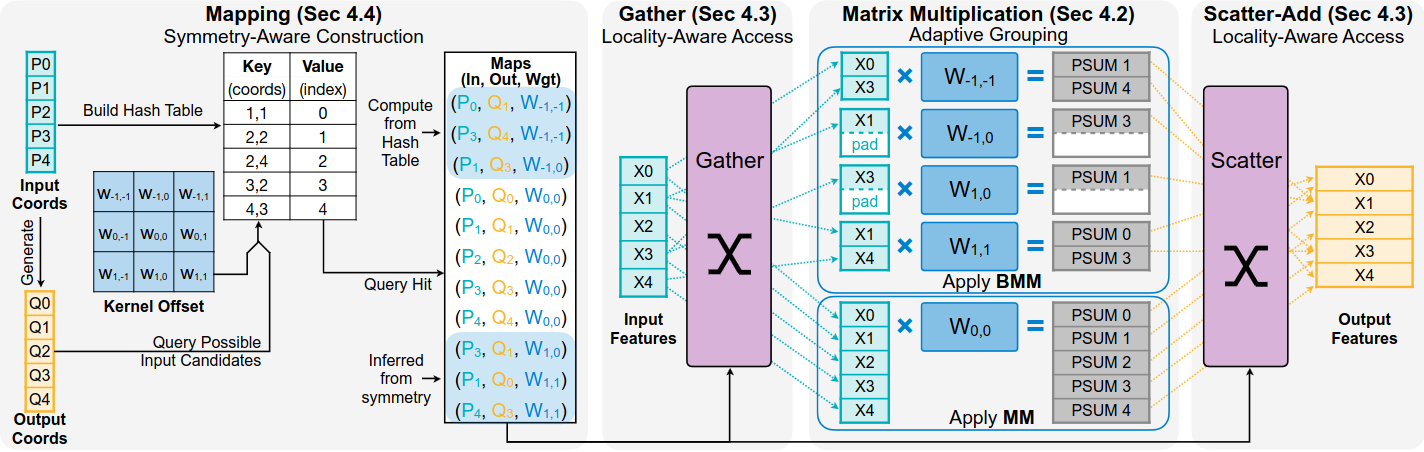
\includegraphics[width=0.90\linewidth]{figures/Torchsparse-hash.png}
    \caption{Torchsparse hashing explanation}
    \label{hashing-explanatoon}
\end{figure*}
Profiling the computation time of each specific CUDA operation showed that most of the time is spent on generating the hashmaps. It was found that one hash map needs to be generated for each input,  as well as for each change in stride; as a stride lengths higher than 1 changes the dimensions of the input and thus a new hashing operation needs to be performed. In figure \ref{hashing-explanatoon} an overview is given of the operations performed by Torchsparse. First an overview is given of the input indices, upon which hashing is performed, followed by a scatter operation to get back the desired output. 

For a low channel count, the hashing step introduces relatively a significant overhead. 

% Furthermore, as was seen throughout the profiling of cuda operations for sparse convolutions the \text{ampere_sgemm_XX} operations were called, whereas for dense onvolutions $aten::mul$ is used. It might be that optimizations for dense multiplicatin have received higher prioritisation as sparse is more niche. This is purely speculative however. 




\begin{table}[ht]
    \centering
    \begin{tabular}{|c|@{\hspace{3pt}}c@{\hspace{3pt}}c@{\hspace{3pt}}c|@{\hspace{3pt}}c@{\hspace{3pt}}c@{\hspace{3pt}}c|@{\hspace{3pt}}c@{\hspace{3pt}}c@{\hspace{3pt}}c|}
        \hline
        Network & \multicolumn{3}{c|}{Minuet [ms]} & \multicolumn{3}{c|}{Dense [ms]} & \multicolumn{3}{c|}{Speedup [-]} \\
        \hline
        Delay & $1$ & $3$ & $5$ & $1$ & $3$ & $5$ & $1$ & $3$ & $5$ \\
        \hline
        \text{[3x3]} & 1.88 & 2.39 & 2.92 & 0.44 & 0.81 & 1.75 & 0.23 & 0.34 & 0.60 \\
        \text{[5x5]} & 2.21 & 3.60 & 5.36 & 0.52 & 1.51 & 3.85 & 0.24 & 0.42 & 0.72 \\
        \text{[7x7]} & 2.82 & 5.63 & 9.18 & 0.63 & 2.31 & 6.40 & 0.22 & 0.41 & 0.70 \\
        \hline
    \end{tabular}
    \caption{Performance comparison by kernel size and temporal depth, time in [s], .......}
    \label{table:corrected_performance}
\end{table}

\subsection{Exploring Use Cases Wherein Sparsity is Beneficial}
\label{Exploring use-cases}

% Discussion on the need for creating a new hashmap with changes in stride or transposed convolutions, and the impact on time.
As was shown in Chapter \ref{Results}, a new hashmap needs to be created whenever the stride of the network changes, or if transposed convolutions are used, which takes a significant amount of time. Minuet partially alleviates this issue by using a faster hashing procedure, but still suffers from the same problems. Based on the results provided in \ref{Results}, the ideal network for leveraging these engines is one which has no changes in stride, a high number of channels, and a large kernel size. Primarily, however, the degree of sparsity from the input is crucial.

% Explanation of the parameter search conducted and the resulting network configurations.
A comprehensive parameter search was conducted, varying the number of filters (represented by the multiplication factor which multiplies the hidden layers of the model by this factor) up to a final network dimension of (2, 128, 256, 256, 128, 2). Larger kernel sizes and temporal dimensions were found to benefit the most from sparsity. The networks presented are those that demonstrated the best performance under these conditions. Figure \ref{fig:speedup_var_kernel} shows that a combination of large filter counts, increased input sparsity, and larger temporal depth achieves the fastest performance relative to dense convolutions. Additionally, the results for a network without changes in dimension (keeping all strides equal to 1) are shown in Figure \ref{fig:kernel_size}. Only the speedup numbers are presented for brevity; however, the full results can be seen in Appendix B.

\begin{table}[ht]
    \centering
    \begin{tabular}{|c|@{\hspace{3pt}}c@{\hspace{3pt}}c@{\hspace{3pt}}c|@{\hspace{3pt}}c@{\hspace{3pt}}c@{\hspace{3pt}}c|@{\hspace{3pt}}c@{\hspace{3pt}}c@{\hspace{3pt}}c|}
        \hline
        Kernel size: & \multicolumn{3}{c|}{[3,3,3]} & \multicolumn{3}{c|}{[3,5,5]} & \multicolumn{3}{c|}{[5,5,5]} \\
        \hline
        \( S \): & $1$ & $5$ & $10$ & $1$ & $5$ & $10$ & $1$ & $5$ & $10$ \\
        \hline
        \( M \): 1 & 0.34 & 0.38 & 0.42 & 0.42 & 0.43 & 0.47 & 0.72 & 0.80 & 0.82 \\
        \( M \): 2 & 0.36 & 0.37 & 0.40 & 0.34 & 0.37 & 0.39 & 0.43 & 0.53 & 0.56 \\
        \( M \): 4 & 0.52 & 0.58 & 0.62 & 0.55 & 0.71 & 0.78 & 0.69 & 1.05 & 1.22 \\
        \( M \): 8 & 0.99 & 1.35 & 1.54 & 1.04 & 1.63 & 2.01 & 1.28 & 2.35 & 3.10 \\
        \hline
    \end{tabular}
    \caption{\( S \) denotes the sparsification factor, with \( S = 1 \) as the baseline and \( S = 10 \) indicating a tenfold increase in sparsity. \( M \) represents the multiplication factor for the number of channels or convolution filters.}
    \label{table:performance_stride_122}
\end{table}

% Table showing performance results for networks without downsampling layers.
\begin{table}[ht]
    \centering
    \begin{tabular}{|c|@{\hspace{3pt}}c@{\hspace{3pt}}c@{\hspace{3pt}}c|@{\hspace{3pt}}c@{\hspace{3pt}}c@{\hspace{3pt}}c|@{\hspace{3pt}}c@{\hspace{3pt}}c@{\hspace{3pt}}c|}
        \hline
        Kernel size: & \multicolumn{3}{c|}{[3,3,3]} & \multicolumn{3}{c|}{[3,5,5]} & \multicolumn{3}{c|}{[5,5,5]} \\
        \hline
        \( S \): & $1$ & $5$ & $10$ & $1$ & $5$ & $10$ & $1$ & $5$ & $10$ \\
        \hline
        \( M \): 1 & 0.98 & 1.07 & 1.09 & 3.06 & 4.11 & 4.18 & 1.88 & 3.30 & 3.64 \\
        \( M \): 2 & 1.20 & 1.64 & 1.66 & 1.30 & 2.01 & 2.05 & 1.32 & 3.19 & 3.53 \\
        \( M \): 4 & 1.70 & 3.65 & 3.71 & 1.88 & 5.38 & 5.72 & 2.31 & 8.00 & 10.26 \\
        \( M \): 8 & 2.69 & 9.93 & 10.61 & 2.78 & 11.80 & 14.79 & 3.24 & 15.58 & 22.26 \\
        \hline
    \end{tabular}
    \caption{Performance results for networks without downsampling layers.}
    \label{table:performance_stride_111}
\end{table}

% Investigation of the impact of the number of channels on performance.
\subsection{Number of Channels}
\label{number_of_channels}
As shown in Figure \ref{fig:speedup_var_kernel}, a substantially higher number of channels increases the computation time for dense convolutions significantly, yet only marginally for sparse networks. A closer inspection reveals that the number of kernel operations only marginally increases, but the operations take significantly longer.

\begin{figure}[h!]
    \centering
    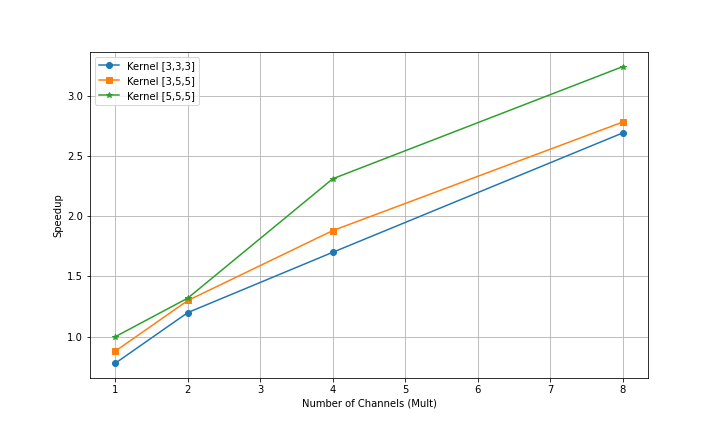
\includegraphics[width=\linewidth]{figures/Plots/speedup_var_kernel_122+step1.png}
    \caption{Speedup vs. Number of Channels for Different Kernels [3,3,3], [3,5,5], and [5,5,5].}
    \label{fig:speedup_var_kernel}
\end{figure}

% Analysis of the impact of not using downsampling layers on sparse network performance.
\subsection{No Downsampling}
\label{no_downsampling}
As shown in Figure \ref{fig:kernel_size}, using strides unequal to 1 results in large computational overhead for sparse networks, as new mapping steps have to be performed and new memory writes are required. The FireNet architecture was analyzed instead. The difference is especially pronounced when compared to dense networks, which are much faster due to the smaller number of convolutions.

\begin{figure}[h!]
    \centering
    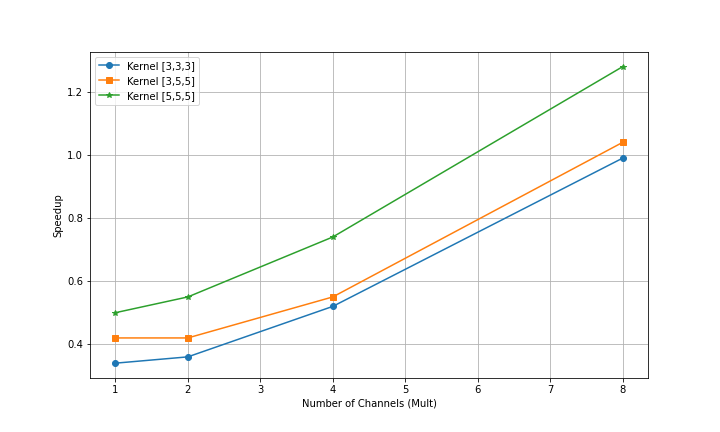
\includegraphics[width=\linewidth]{figures/Plots/kernel_size(1,1,1).png}
    \caption{Speedup vs. Number of Channels for Different Kernels [3,3,3], [3,5,5], and [5,5,5].}
    \label{fig:kernel_size}
\end{figure}

% Discussion on the impact of sparsity percentage on network performance.
\subsection{Sparsity Percentage}
\label{sparsity_percentage}
The sorted index was adapted by using `index = index[::STEP]`, with `STEP` being the number of skips in the coordinate data, effectively reducing the sparsity by a factor equal to this number. As sparse libraries are intended for data with sparsity levels of around 99\% \cite{yang2023minuet}, the input data was modified to more closely reflect this number.

\begin{figure}[h!]
    \centering
    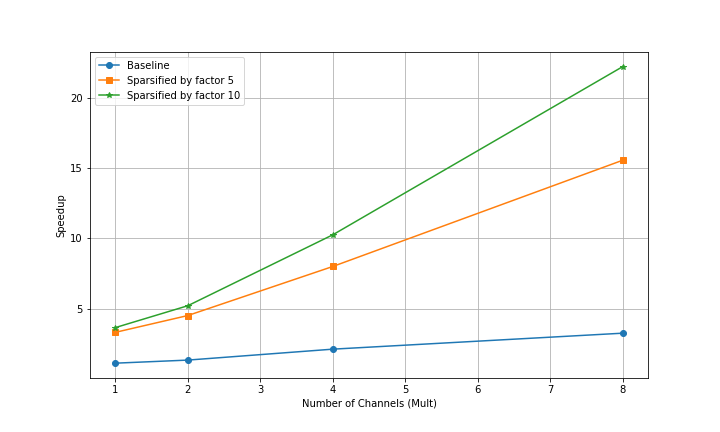
\includegraphics[width=\linewidth]{figures/Plots/speedup_var_sparsity_555+(1,1,1).png}
    \caption{Speedup vs. Number of Channels for Kernel [5,5,5] at Different Sparsification Steps.}
    \label{fig:speedup_var_sparsity}
\end{figure}

% Summary of the final results and observations.
\subsection{Final Results}
\label{final_results}
The final results of our investigation demonstrate the significant potential of sparsity in convolutional neural networks under specific conditions. Networks with no changes in stride, high numbers of channels, and large kernel sizes, particularly those maintaining a high degree of input sparsity, exhibit substantial speedups. The comprehensive parameter search highlights the configurations where sparse networks can significantly outperform their dense counterparts.

\section{Conclusion}
\label{Conclusion}
It was found that for a small network (32 bottleneck channels) and input sparsity levels of about 85\%, dense convolution is faster than sparse convolution, even without accounting for the additional overhead in generating sparse tensors and converting the output data back to their original snoted that this process incurs significant computational costs,
and is assumed to be performed throughout the data preparation step (before training). The validity of this assumption
will be discussed in 5.

However, the research identified specific scenarios where sparse convolutional libraries provide potential performance advantages:
\begin{itemize}
    \item \textbf{Channel Density:} Networks with a higher number of channels benefit more from sparse convolutions due to the reduced computational load relative to dense networks.
    \item \textbf{Network Architecture:} Architectures like FireNet, which preserve input dimensions across layers, exhibit fewer dimensional changes and therefore require fewer hashmap generations. This efficiency reduces the overhead typically associated with sparse networks.
    \item \textbf{Data Sparsity:} The benefits of sparse convolutions scale with the level of data sparsity. The findings suggest that for inputs with a sparsity level of 99\% or greater, sparse networks perform more efficiently than their dense counterparts.
\end{itemize}

In conclusion, dense GEMM appears to be sufficiently optimized such that even for a large number of zeroes in the input data dense convolutions outperform their sparse counterpart. For neural networks with a large number of filters, a low number of dimensional changes, sparse inputs (preferably at least 99\%), the performance benefits of using Minuet can outweigh the drawbacks. 

\section{Discussion}
\label{discussion}

Still premature. Minuet super new and does not yet support training. Limited number of activation function (relu, relu6 signmoid) for example. Others can be made by writing custom cuda kernels but this shows it's not an easy plug and play. 

Instead of sparsity, also other approaches such as torch.compile or torch.autocast may be of use 

Assumption that for example 140 sequences of event data can be generated. The assumption is that this can be done beforehand, yet this step would have to be performed whenever the batch size or sequence length changes, limited adaptability. However, even when this is changed and the sparse tensors for the input have to be generated, it can still be seen as negligible in comparison to a full training run consisting of hundreds of epochs. 

Assumption that tensors can be made beforehand
Network will change so hashing maps can not be made beforehand

Output is sparse, if dense optical flow is desired then this step will also cost some time

In terms of code complexity, sparse neural networks can be unintuitive to work with, and requires a rewrite of the input data into SparseTensor objects, rewriting the network architecture. Also still in development, for example no tile sizes of 48 etc supported limiting flexibility of the network, and custom activations such as tanh are also not yet supported. Can be done cuda but different framework. 

\section{Future Work}
The input for the network consists of activations by event cameras which per pixel is 0 when no (significant) change in brightness has been detected, and 1 otherwise. As event data gets captured at a higher rate than it is processed, some of these activations get concatinated together such that also 2's and 3'd are present in the EVIMO2 dataset. However, for the (majority) inputs of 1 for each active input site in theory only addition is needed to sum up the weights of the kernel instead of multiplication. This however would require an entirely novel approach and custom CUDA kernels. 

As the Torchsparse++ mapping step is significantly slower using Minuet is much preferred. However, it only provides support for inference and not yet for performing the gradient calculations required for training. Once this has been added also a full comparison of training times can be performed. 

Next to profiling CUDA operations, a count of the number of FLOPS is also provided by the native pytorch profiler. This is still an experimental feature however, and I was not able to compare the number of operations for both networks as no explicit calls to aten::mul were made. Only for Torchsparse was this the case (with around 100.000.000 flops per forward pass). 

\section*{Acknowledgements}
I would like to thank Jesse Hagenaars for his inputs and valuable discussions. Furthermore I would like to thank the TU Delft MAVLab for providing access to their A100 GPU for testing the various hypotheses. Lastly, I would like to thank Guide de Croon and Christophe de Wagter for their lectures on optical flow, and Jan van Gemert for teachings on neural networks. 


\bibliography{Bibliography}

%\appendix
%\subsection{Sparse Matrices}
Sparse matrices predominantly contain zero elements. Storing these explicitly is inefficient, leading to the development of compact storage schemes. Two popular formats are the Coordinate (COO) and the Compressed Sparse Row (CSR) formats.

\textbf{Coordinate (COO) Format}:
A sparse matrix in COO format is represented using three one-dimensional arrays:
\begin{itemize}
    \item \textit{rows}: Row indices of non-zero elements.
    \item \textit{cols}: Column indices of non-zero elements.
    \item \textit{vals}: Non-zero elements.
\end{itemize}
For any index $k$, the matrix element is $(\textit{rows}[k], \textit{cols}[k]) = \textit{vals}[k]$.


\subsection{Evimo5 Dataset}
Evimo is a toolkit for fusing data streams from multiple cameras (event-based, rgb or potentially any other kind of visual sensor) with a motion capture system in a AR-like fashion to automatically generate ground truth annotations for motion, depth and scene segmentation (both motion or semantic). The toolkit uses static 3D scans of the objects on the scene to achieve this goal - the objects and cameras are fitted with motion capture markers and the simulated ground truth is overlaid on the real data from sensors.


\end{document}

